\documentclass{article}
\usepackage[utf8]{inputenc}
\usepackage{amsmath}
\usepackage{amssymb}
\usepackage{enumitem}
\usepackage{graphicx}
\usepackage[margin=2.5cm]{geometry}
\usepackage{subcaption}
\usepackage{setspace}
\usepackage{pgfplots}

\title{Gabarito - Lista 1 - Estatística I}
\date{}

\begin{document}
\onehalfspacing
\maketitle

\section*{Questão 9}

\begin{enumerate}[label=(\alph*), start=1]
    \item Primeiro, vamos construir as tabelas com as densidades. Em seguida, podemos construir o histograma.
    
    \textbf{Zona Urbana}
    
    \begin{center}
    \begin{tabular}{|c|c|c|c|c|c|}
    \hline
    Classe de Aluguéis & Frequência $n_i$ & Amplitude $\Delta i$ & Densidade $\frac{n_i}{\Delta i}$ & Proporção $f_i$ & Densidade $f/\Delta i_i$ \\
    \hline
    2-3 & 10 & 1 & 10 & 0,050 & 0,050 \\
    3-5 & 40 & 2 & 20 & 0,100 & 0,050 \\
    5-7 & 80 & 2 & 40 & 0,200 & 0,100 \\
    7-10 & 50 & 3 & 16,67 & 0,083 & 0,028 \\
    10-15 & 20 & 5 & 4 & 0,020 & 0,004 \\
    \hline
    Total & 200 & & 1,00 & & \\
    \hline
    \end{tabular}
    \end{center}
    
    \textbf{Zona Rural}
    
    \begin{center}
    \begin{tabular}{|c|c|c|c|c|c|}
    \hline
    Classe de Aluguéis & Frequência $n_i$ & Amplitude $\Delta i$ & Densidade $\frac{n_i}{\Delta i}$ & Proporção $f_i$ & Densidade $f/\Delta i_i$ \\
    \hline
    2-3 & 30 & 1 & 30 & 0,300 & 0,300 \\
    3-5 & 50 & 2 & 25 & 0,250 & 0,125 \\
    5-7 & 15 & 2 & 7,5 & 0,075 & 0,038 \\
    7-10 & 5 & 3 & 1,67 & 0,017 & 0,006 \\
    10-15 & 0 & 5 & 0 & 0,000 & 0,000 \\
    \hline
    Total & 100 & & 1,00 & & \\
    \hline
    \end{tabular}
    \end{center}
    
   O histograma da densidade $f/\Delta i_i$ por classes de aluguéis é mostrado abaixo:
    
    \begin{center}
        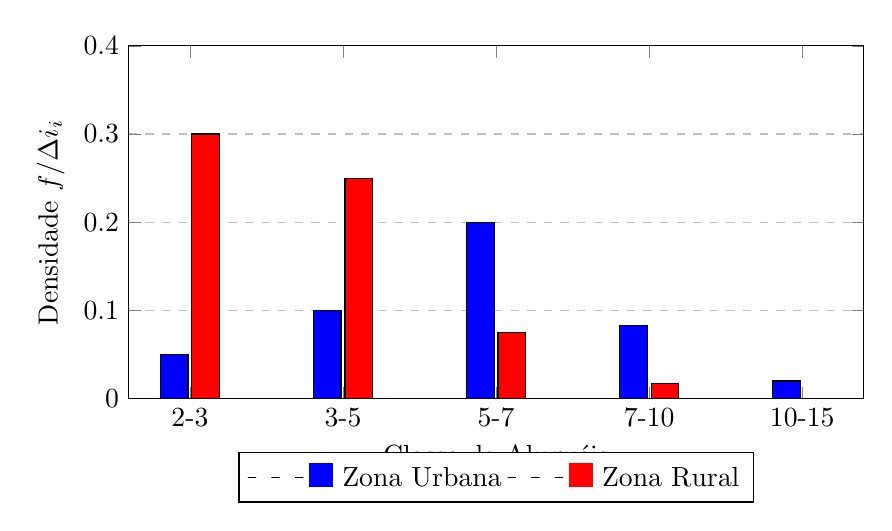
\begin{tikzpicture}
            \begin{axis}[
                width=0.9\textwidth, % Alterado o tamanho do gráfico
                height=0.5\textwidth, % Alterado o tamanho do gráfico
                xlabel={Classe de Aluguéis},
                ylabel={Densidade $f/\Delta i_i$},
                ymin=0,
                ymax=0.4,
                ytick={0,0.1,...,0.4},
                xtick=data,
                xticklabels={2-3, 3-5, 5-7, 7-10, 10-15},
                bar width=0.35cm,
                legend style={at={(0.5,-0.15)}, anchor=north, legend columns=-1},
                enlarge x limits=0.1,
                ymajorgrids=true,
                grid style=dashed,
            ]
            \addplot[ybar, fill=blue, bar shift=-0.2cm] coordinates {
                (1, 0.050)
                (2, 0.100)
                (3, 0.200)
                (4, 0.083)
                (5, 0.020)
            };
            \addplot[ybar, fill=red, bar shift=0.2cm] coordinates {
                (1, 0.300)
                (2, 0.250)
                (3, 0.075)
                (4, 0.017)
                (5, 0.000)
            };
            \legend{{\color{blue}\rule{0.3cm}{0.3cm}} Zona Urbana, {\color{red}\rule{0.3cm}{0.3cm}} Zona Rural}
            \end{axis}
        \end{tikzpicture}
    \end{center}
    
\item A densidade de frequência no gráfico da zona urbana revela que a classe de aluguéis predominante é 5-7, indicando uma distribuição mais equilibrada de valores de aluguéis, com uma concentração considerável nessa faixa. No entanto, no caso das famílias provenientes da zona rural, a classe predominante de aluguéis é 2-3, evidenciando uma predominância de valores mais baixos entre a população observada. Notavelmente, a distribuição da densidade das classes de aluguéis é mais simétrica em torno da classe 5-7, onde se encontra a mediana, na zona urbana, enquanto é mais assimétrica para a esquerda na zona rural. Isso sugere uma disparidade significativa nos custos de aluguel entre as áreas urbanas e rurais, com uma distribuição mais uniforme de valores na zona urbana e uma maior concentração de valores mais baixos na zona rural.

\end{enumerate}

\section*{Questão 1}

\begin{table}[htb]
    \centering
    \begin{tabular}{|c|c|}
        \hline
        \textbf{Frequência} & \textbf{Valor} \\
        \hline
        0 & 25 \\
        1 & 20 \\
        2 & 3 \\
        3 & 1 \\
        4 & 1 \\
        \hline
    \end{tabular}
    \caption{Frequência de valores}
    \label{tab:frequencia_valores}
\end{table}

\begin{enumerate}

    \item[(a)] O número médio de erros por página é calculado pela fórmula:
    \[
    \bar{x} = \frac{1}{50} \sum_{i=1}^{50} x_i = \frac{1}{50} \left( 0 \times 25 + 1 \times 20 + 2 \times 3 + 3 \times 1 + 4 \times 1 \right) = \frac{33}{50} = 0,66
    \]
    
    Portanto, o número médio de erros por página é aproximadamente $0,66$.
    
    \item[(b)] Para determinar o número mediano, vamos primeiro ordenar os valores do menor para o maior. Dados os valores:

\[ 0, 0, 0, \dots, 0, 1, 1, \dots, 1, 2, 2, \dots, 2, 3, 4 \]

Como o tamanho da amostra é $50$, ou seja, é par, a mediana amostral é dada pela média dos dois valores do meio:

\[ \text{md} = \frac{x_{25} + x_{26}}{2} = \frac{0 + 1}{2} = 0,5 \]

\item[(c)] O desvio padrão amostral é dado por:

\[
S_x = \sqrt{\frac{1}{50 - 1} \sum_{i=1}^{50} (x_i - \bar{x})^2}
\]
\\
\[
= \sqrt{\frac{1}{49} \left[ 25(0 - 1.32)^2 + 20(1 - 1.32)^2 + 3(2 - 1.32)^2 + 1(3 - 1.32)^2 + 1(4 - 1.32)^2 \right]} \approx 0,8478.
\]

Portanto, o desvio padrão é aproximadamente $0,8478$.

\item[(d)] Vamos agora criar uma representação gráfica para a distribuição dos erros por página. Abaixo está o histograma com as frequências e densidades correspondentes.


\begin{figure}[h!]
    \centering
    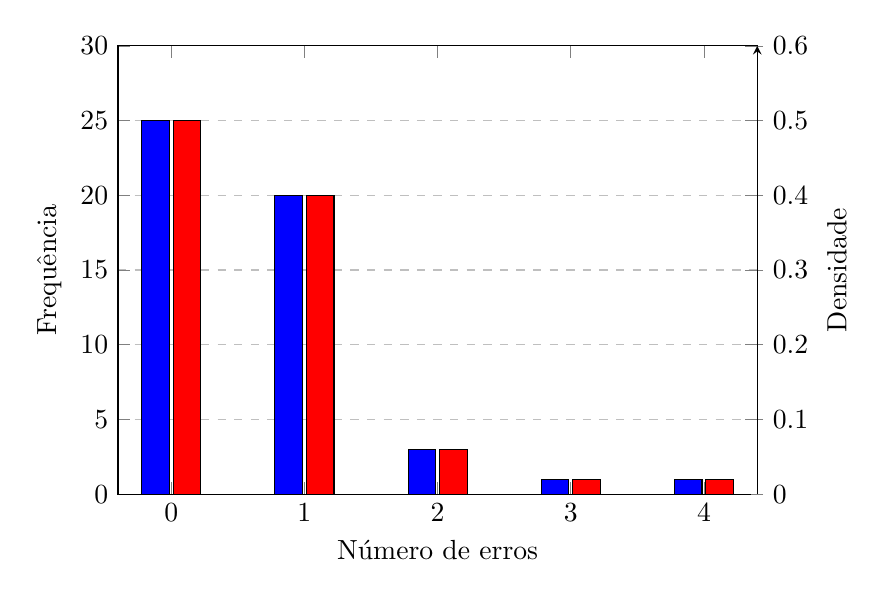
\begin{tikzpicture}
        \begin{axis}[
            width=0.8\textwidth,
            height=0.6\textwidth,
            xlabel={Número de erros},
            ylabel style={align=center},
            ylabel={Frequência},
            ymin=0,
            ymax=30,
            ytick={0,5,...,30},
            xtick=data,
            xticklabels={0,1,2,3,4},
            bar width=0.35cm,
            legend style={at={(0.5,-0.15)}, anchor=north, legend columns=-1},
            enlarge x limits=0.1,
            ymajorgrids=true,
            grid style=dashed,
        ]
        \addplot[ybar, fill=blue, bar shift=-0.2cm] coordinates {
            (0, 25)
            (1, 20)
            (2, 3)
            (3, 1)
            (4, 1)
        };
        \end{axis}
        \begin{axis}[
            width=0.8\textwidth,
            height=0.6\textwidth,
            axis y line=right,
            axis x line=none,
            ylabel style={align=center},
            ylabel={Densidade},
            ymin=0,
            ymax=0.6,
            yticklabel style={/pgf/number format/fixed},
            ytick={0,0.1,...,0.6},
        ]
        \addplot[ybar, fill=red, bar shift=0.2cm] coordinates {
            (0, 0.50)
            (1, 0.40)
            (2, 0.06)
            (3, 0.02)
            (4, 0.02)
        };
        \end{axis}
    \end{tikzpicture}
    \caption{Histograma de frequência e densidade dos erros por página}
    \label{fig:histograma_frequencia_densidade}
\end{figure}



\item[(e)] Partindo do pressuposto de que a nossa amostra é não viesada (por exemplo, se escolhermos só
páginas com imagens, isto é, haveria menos palavras por página, subestimando o número de erros),
espera-se que encontremos 330 erros nas 500 páginas (lembre-se que a média amostral de erros é 0,66
por página). 

\end{enumerate}


\section*{Questão 2}

As taxas de juros recebidas por 10 ações durante um certo período foram (medidas em porcentagem):
$2.59; 2.64; 2.60; 2.62; 2.57; 2.55; 2.61; 2.50; 2.63; 2.64$. Calcule a média, a mediana e o desvio padrão.

\textbf{Considerando os dados como uma amostra:}

\begin{itemize}
    \item Média amostral:
    \[
    \bar{r} = \frac{2.59 + 2.64 + 2.60 + 2.62 + 2.57 + 2.55 + 2.61 + 2.50 + 2.63 + 2.64}{10} = 2.595
    \]
    
    \item Mediana amostral:
    \[
    \text{md} = \frac{2.6 + 2.61}{2} = 2.605
    \]
    
    \item Variância amostral:
    \[
    \begin{split}
    S^2 = \frac{1}{10 - 1} & \left[ (2.5 - 2.595)^2 + (2.55 - 2.595)^2 + (2.57 - 2.595)^2 + (2.59 - 2.595)^2 \right. \\
    & \left. + (2.6 - 2.595)^2 + (2.61 - 2.595)^2 + (2.62 - 2.595)^2 + (2.63 - 2.595)^2 \right. \\
    & \left. + (2.64 - 2.595)^2 + (2.64 - 2.595)^2 \right] \approx 0.001983
    \end{split}
    \]
    
    \item Desvio padrão amostral:
    \[
    S \approx \sqrt{0.001983} \approx 0.0445
    \]
\end{itemize}

\textbf{Considerando os dados como uma população:}

\begin{itemize}
    \item Variância populacional:
    \[
    \begin{split}
    \sigma^2 = \frac{1}{10} & \left[ (2.5 - 2.595)^2 + (2.55 - 2.595)^2 + (2.57 - 2.595)^2 + (2.59 - 2.595)^2 \right. \\
    & \left. + (2.6 - 2.595)^2 + (2.61 - 2.595)^2 + (2.62 - 2.595)^2 + (2.63 - 2.595)^2 \right. \\
    & \left. + (2.64 - 2.595)^2 + (2.64 - 2.595)^2 \right] \approx 0.001785
    \end{split}
    \]
    
    \item Desvio padrão populacional:
    \[
    \sigma \approx \sqrt{0.001785} \approx 0.0422
    \]
\end{itemize}

\begin{figure}[h]
    \centering
    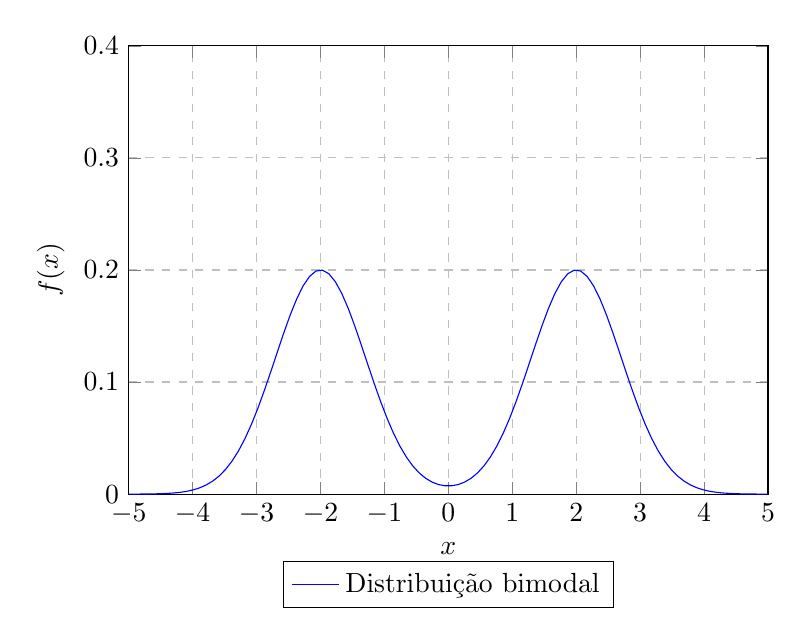
\begin{tikzpicture}
        \begin{axis}[
            domain=-5:5,
            samples=100,
            width=0.8\textwidth,
            height=0.6\textwidth,
            xlabel={$x$},
            ylabel={$f(x)$},
            xmin=-5,
            xmax=5,
            ymin=0,
            ymax=0.4,
            xtick={-5,-4,...,5},
            ytick={0,0.1,...,0.4},
            legend style={at={(0.5,-0.15)}, anchor=north, legend columns=-1},
            grid=both,
            grid style=dashed,
        ]
        \addplot[blue,domain=-5:5] {0.2*exp(-(x+2)^2) + 0.2*exp(-(x-2)^2)};
        \addlegendentry{Distribuição bimodal}
        \end{axis}
    \end{tikzpicture}
    \caption{Distribuição bimodal}
    \label{fig:bimodal_continuous_distribution_same_height}
\end{figure}
    
    
\section*{Questão 5}

A média e a mediana são medidas de posição que fornecem informações sobre onde o centro da distribuição de dados está localizado. No entanto, apenas essas medidas de posição são insuficientes para compreender completamente a natureza da distribuição dos dados. A média é sensível a valores extremos (outliers), o que pode distorcê-la, enquanto a mediana é menos sensível a esses valores atípicos, o que a torna uma medida mais robusta em algumas situações.

No entanto, tanto a média quanto a mediana não fornecem informações sobre a forma da distribuição dos dados, como simetria ou assimetria, nem sobre a dispersão dos dados. Para obter uma compreensão mais completa da distribuição, é necessário considerar medidas adicionais, como a moda, que fornece informações sobre os valores mais frequentes na distribuição. Se houver duas modas, como é o nosso caso, isso indicaria uma distribuição bimodal, sugerindo a presença de dois grupos distintos na amostra.

Portanto, embora a média e a mediana sejam importantes para entender a posição central dos dados, é necessário complementá-las com outras medidas, como a moda, para obter uma compreensão mais completa da distribuição dos dados.

\section*{Questão 6}

\begin{enumerate}
    \item[(a)] A mediana do número de filhos é 2. Isso significa que metade das famílias têm dois filhos ou menos, enquanto a outra metade tem dois filhos ou mais.
    
    \item[(b)] A moda, ou seja, o valor mais frequente, é 2. Isso ocorre porque a maioria das famílias tem dois filhos.
    
    \item[(c)] Para calcular a média, enfrentamos um problema ao considerar o grupo de famílias com "mais que 5" filhos. Sem uma contagem precisa, assumimos que "mais que 5" representa 6 filhos. Assim:
    
    
    \[
    \bar{X} = \frac{0 \times 17 + 1 \times 20 + 2 \times 28 + 3 \times 19 + 4 \times 7 + 5 \times 4 + 6 \times 5}{100} = 2,11,
    \]
    
     Com essa suposição, a média aproximada é 2,11 filhos por família.
\end{enumerate}


\end{document}

